\documentclass[12pt]{report}
\usepackage[a4paper, total={6in, 8in}]{geometry}
\usepackage{amsmath, amsfonts, amsthm, amssymb, fontspec}
\usepackage{graphicx} % Required for inserting images
\usepackage{tabularx}
\usepackage{xcolor} 
\usepackage{quotchap}
\usepackage{anyfontsize}
\usepackage{epigraph}
\setlength{\epigraphwidth}{.5\textwidth}
\usepackage{float}
\usepackage{wrapfig}
\usepackage{hyperref,cleveref,comment}
\hypersetup{colorlinks=true,urlcolor=blue}
\usepackage{mathtools}
\usepackage{titlesec}
\usepackage{verbatim}
\usepackage{appendix}
\usepackage{parskip}
\usepackage[none]{hyphenat}
\usepackage{enumitem}
\usepackage{contour}
\usepackage{ulem}
\usepackage[most]{tcolorbox}
\usepackage{fancyvrb}
\usepackage{lastpage, cancel}
\usepackage{derivative}
\usepackage{newpxtext,newpxmath}


%\usepackage[colorinlistoftodos]{todonotes}

\usepackage[Conny]{fncychap}
%Options: Sonny, Lenny, Glenn, Conny, Rejne, Bjarne, Bjornstrup
\pagenumbering{arabic}
\hypersetup{pdfborder=0 0 0}

\newcommand{\mychapter}[2]{
    \setcounter{chapter}{#1}
    \setcounter{section}{0}
    \chapter*{#2}
    \addcontentsline{toc}{chapter}{#2}
}

% Each week, someone will look at this for the last time, what would the most useful thing they should see? 

% REMEMBER TO PUSH UPDATES TO GITHUB - BE WARY OF MERGE CONFLICTS!! 


\begin{document}



\title{A Field Guide to Mathematics at Southampton}
\author{
  1st Year Student (25/26) 
}

\maketitle

% Answering - what on earth this is 
\chapter*{What This Guide Is (and Isn't)} 

% Write the abstract/introduction twice - once at the start, and once at the end. Right now, as I'm working on this, I will not be checking my writing as I write without consciously thinking about it.. the second I start acutally thinking I will stop writing. Editing will come later, or else this will end up way too many words, "Kill your darlings, kill your darlings, even when it breaks your egocentric little scribbler's heart"

\epigraph{Mathematics is one of the most beautiful things in the world and it brings joy and fulfilment and frustration in equal measure, and what more could you possibly want out of life}
{\textit{Graham A. Niblo}}


% This is not a maths textbook, so don't read it like one. Think of it as a transition guide from school to university mathematics. This guide is written by a first-year student, and intended for first year students as a personal reflection of how the transition to maths felt like. 

% Talk about what the guide covers briefly, it's designed to address FAQs and confusions regarindg the subject here. 

% In the chapters that follow, I'll talk about the mindset shift itself, alongside making the most of lectures and resources, the temptation to outsource thinking, dealing with exams, time management, and in general, things I wish I had known before I got here.

This is not a Maths textbook.

It won’t teach you how to compute an integral or prove a theorem step by step. It won’t replace lectures, problem sheets, or workshops, and it isn’t a shortcut through the degree. Think of it instead as a transition guide, written from inside the experience and not from the other side of it.

There are countless books and resources about transitioning to university mathematics. However, most I found were written by people who had already finished the journey and looked back with clarity and hindsight, so I wanted something written from inside the process, something honest that reflects what progress feels like while it's happening. 

This guide isn’t here to solve all possible problems you may encounter, but it's here to help you think about how you learn. It attempts to articulate the parts of the degree that may be scattered across multiple places. You don’t need to read it all at once. Some chapters might resonate immediately, others might make more sense later.

In the chapters that follow, I’ll talk about:
\begin{itemize}
    \item The shift from school mathematics to university mathematics
    \item Types of classes and coursework 
    \item Workshops and supporting resources 
    \item How to approach problem solving 
    \item Revision, exams, and time management 
    \item Outsourcing thinking 
    \item Asking for help and providing feedback 
\end{itemize}

I've also scattered a few \textbf{\href{https://xkcd.com/}{xkcd}} references along the way because sometimes, a well-timed joke explains the mood of mathematics better than a paragraph every could. 

Not everyone signs up for a maths degree wanting a philosophical reflection on learning, and that's completely fine. But if you want to care about how you learn, and not just what you learn, I hope this helps.

\begin{figure}[H]
    \centering
    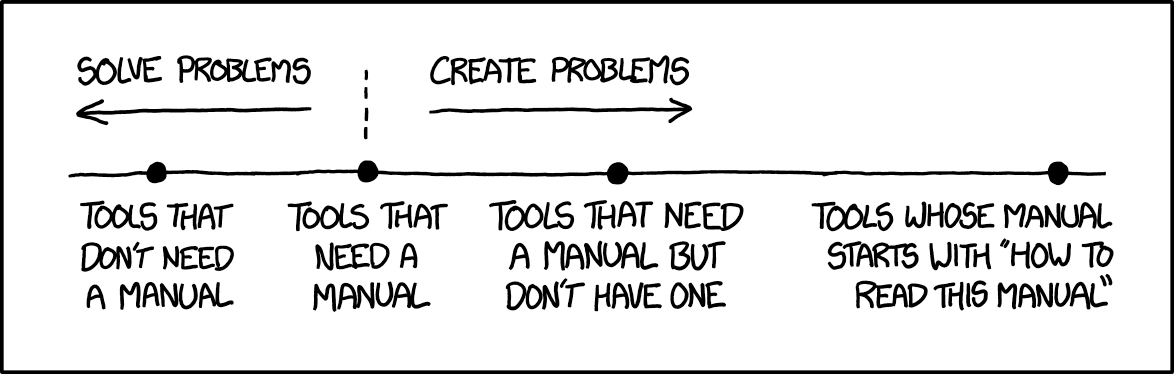
\includegraphics[width=0.5\linewidth]{xkcd/manuels.png}
    \caption{\textbf{\href{https://xkcd.com/1343/}{Manuels}}}
\end{figure}

%  section on terminology and acronynms like PAT, SSLC, SUSU, CATS, SUMS, SUAS, coursework, office hours, blackboard/moodle, formatie/summative, etc? 


\setcounter{tocdepth}{1}
\tableofcontents

% selection of xkcd 

\mychapter{1}{The Jump To University}
\epigraph{I was born not knowing and have only had a little time to change that}
{\textit{Richard P. Feynman}}

\section{The Mindset Shift}

At school, I became used to understanding things quickly. If I didn’t understand something in class, I could by the end of the lesson. And if I didn’t, I could do a couple questions and it would click. University maths felt different almost immediately.

Having worked at department offer holder days, one of the most common questions I get asked is: \textit{`What’s the jump actually like? Is it just harder? Is it just more content?'}

My honest answer has been, and still is: it’s just different.

\section{What Actually Changes}

The most noticeable change is that you don’t understand things straight away. I remember hearing this at open days but I don't think I understood this until experienced it firsthand. 

At school, not understanding meant you needed more practice. University requires need more time, reflection, even different way of thinking about the problem. This can be particularly difficult if you’re used to being `the maths person', or the one who usually gets it first, so change isn’t just academic, it’s psychological.

In many subjects or courses, you can revise by memorising key ideas, reading around the topic or absorbing information repeatedly until it sticks. Mathematics doesn't work like that. You can't (always) memorise your way into deep understanding or skim a proof and expect it to feel natural. You can't treat definitions and just some vocabulary words and hope they'll make sense. 
 
\section{Redefining Understanding}

If you ever feel confused or find yourself struggling, rest assured, you're not alone. It's incredibly common, normal, and all part of the process. A lot of the difficulty comes not from the material itself, but from the expectations you might place on yourself. 

Mathematics is a conceptually difficult subject. If you approach each lecture or assignment with the mindset that you're expected to understand everything, or feeling confused means you're not good enough, the delay or lack of those things can feel like failure. 

The challenging part is letting go of the need to understand everything immediately. This doesn't mean lowering standards, but adjusting expectations. Understanding at this level takes time and sitting with ideas that don’t immediately make sense, as well as trying approaches that don’t work and getting used to not always being the fastest or most confident in the room.


\begin{figure}[H]
    \centering
    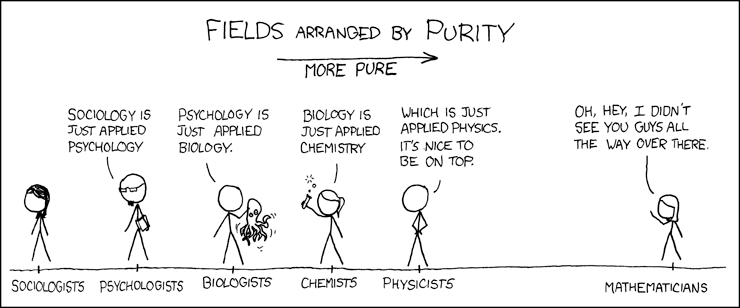
\includegraphics[width=0.5\linewidth]{xkcd/purity.png}
    \caption{\textbf{\href{https://xkcd.com/435/}{Purity}}}
\end{figure}


\mychapter{2}{Lectures and Coursework}
\epigraph{The brain is a wonderful organ; it starts working the moment you get up in the morning and does not stop until you get into the office}
{\textit{Robert Frost}}

\section{Overview}

% Talk about how lectures are gonna be different to classroom learning and how to deal with that, how the material comes up quite fast. 
% how many lectures per module 
% what is the general structure like of lectures 
% Note on notes being provided beforehand + other resources 
% how long they are 

In your first year, your typical week will consist of a mixture of lectures, seminars, tutorials, problem classes, labs, coursework and workshops. 

For example, in my first semester, I had four modules consisting of three lectures a week and a problem class lasting 45 minutes. Alongside this, I had Core Skills and workshop sessions, which left me plenty of time to be involved in a range of clubs and societies.

\subsection{Core Skills}
% info on core skills module? - what it's about..? - basically mention infor that is alreaady on blackboard 
Core Skills is a compulsory and non-credited module that is taken by everyone in the first year. 

As part of the module, you will have to pass two Core Maths Skills Tests, one per semester. The tests gives you a way of making sure you have these skills right from the beginning of your study (Semester 1) and as your study progresses (Semester 2). Both of these are online exams that can be taken repeatedly until you have passed. 

There are also scheduled sessions on employability and digital skills. These sessions are designed to maximise your digital literacy and employment prospects during and after your degree. 
% links to careers page, etc. 


\subsection{Problem Classes}
% What they are - how to make the most of them 
% Try and have a look at the problems beforehand 
% what is the mode up-to-date info on this? 

Each module will have a weekly problem class. These are quite different from lectures. Instead of listening to new material being introduced, the focus is on working through questions and understanding how the ideas from the lectures actually get used.

The exact format can vary slightly between modules and lecturers. Sometimes the lecturer will go through selected problems on the board, sometimes students will suggest questions they want to see explained, and sometimes you go might go through some coursework questions. 

One of the most important thing you can do to make problem classes useful is look at the problems beforehand. If you walk into a problem class having never seen the sheet before, it’s much harder to follow what’s going on and becomes easy to just copy down solutions without really understanding them.

\section{Online Learning Tools}

% timetable can be found on Seats and on blackboard - useful to link timetable to google calendar or something equivalent. 
% Check in with Seats - QR code or the seats code will usually be given start of the lecture  - keeps a good track of attendance 


You'll become familiar with a variety of names very quickly: \textbf{Blackboard}, \textbf{Seats}, and \textbf{Panopto}

Blackboard is the university's online learning platform where lectures notes are uploaded, announcements are posted and the coursework and recordings are stored. If something official happens in the module, it will most likely appear there. It's useful having a quick look at notes before the lecture if you can, even just seeing the headings can make it much easier to follow what’s happening when you’re sitting in the lecture hall.

Panopto is where you can access lecture recordings, including historical recordings. 

One of the most useful things you can do in the first week is link your timetable to your own calender, whether that's Google Calendar or something equivalent. Remember that universities will not chase you the way school did. There are no bells and no-one reminds you every morning where you're supposed to me, so the responsibility shifts to you. 

Seats is the system used for timetabling and attendance. It shows your lecture locations, times, and room numbers. It's also how attendance is recorded. At the start of lectures, a QR or Seats code will be displayed on the board which students can scan or type to register their attendance on the app. 

\section{Recorded Doesn't Mean Optional}

You will quickly realise that most lectures are recorded, and at some point you might be temped to think, `I can just watch it later', especially on a cold and rainy morning, or after a late night, or when the idea of sitting in a lecture feels mildly exhausting. 

I cannot stress this enough, but being physically present in a lecture matters more than you think. When you are in the room, you are less likely to pause a video and get distracted by your phone. You are also less likely to tell yourself that you'll `finish it later' and risk not coming back to it. You are more likely to stay with the explanations as they unfold, even if you don't fully understand them yet. You hear the throwaway comments that never make it into typed notes, and pick up on the emphasis in the lecturer's voice when they say something is important, and that emphasis stays with you. 

There is also something about the collective focus that recordings cannot replicate. Sitting in a room full of people who are all attempting to follow the same proof creates a concentration that watching it alone at 1.5x speed, half distracted cannot compete with. In addition to that, you are able to ask questions during or after the lecture if you attend in person. 

Recordings are useful, in fact, they are incredibly useful for revision or revisiting a proof if that felt unclear the first time. They are a safety net, but not a replacement for showing up. 

\section{Catching Up On Lectures}

At some point, you may very well miss a lecture. Maybe you were ill, overslept, or just needed a morning off. It happens, and one missed lecture is not a crisis.

The trick to avoid spiralling is to catch up quickly. If you miss a lecture, watch the recording within a day or two while the topic and notation is still familiar. Don't let it all pile onto future you.  

% SHORT ASIDE ON FUNNY WAY OF GETTING YOURSELF BACK INTO FOCUS, LIKE HOW I HAD TO BE IN THE GYM DOING A 2 hr ZONE 2 RIDE WHILE WATCHING CALC RECORDINGS. 

When you do catch up, don't treat the recording like a background noise. Try to follow the argument yourself. Stop and ask whether you understand what each part is doing. 

You won't always find it easy to sit down and follow a lecture, I certainly couldn't at all times. In fact, at one point in Semester 2, I'd go to the gym on weekends, get on one of the stationary bikes and rewatch my Calculus lectures while cycling. I wasn't taking notes or anything, but I was surprisingly engaged with the material. There isn't a single `correct' way to study and sometimes, the hardest part is just getting yourself to engage with the material at tall, so if something slightly unconventional helps you do that, it's probably worth trying. 

\section{Asking questions}
% Why it's a good thing - link back to being present in person 
% Addressing fear and embarassemtn of asking questions in lectures 

If you ever find yourself sitting in a lecture room, slightly unsure about a definition or confused about some step in a proof, and you look around the room and everyone else looks calm, and you might think, `Maybe it's just me'. 

It almost never is. Most people are running through the same internal debate of `Is this worth asking? Is this obvious? Is this too stupid of a question?', etc. 

Questions like `How did we go from Line 1 to Line 2 of this proof', or `Is there an example where this conditions fails?' are perfectly good questions to ask in lecture. There are no stupid questions. 

By asking questions, you benefit yourself and others, including the lecturer. Learning mathematics is a process and asking questions is part of that process. If asking during the lecture feels too intimidating, most lecturer's are more than happy for students to ask them at the end of the lecture, or during office hours and workshops. 

\subsection{Talking in lectures}
% Basically - pls shut the fuck up and dont' talk over lectueres, it's rude, distruptive, interrupts other people's focus 

Lectures are shared learning spaces and everyone in the room is trying to concentrate on the same material. It might seem harmless to chat quietly during a lecture, but even small conversations can be a distracting for the people sitting nearby especially with an attention demanding subject like maths. 

More importantly, it's also a matter of respect. The lecturer has prepared the material and everyone else in the room has chosen to be there to learn. Talking over them or holding side conversations can come across as rude even if that isn't the intention. 

If you want to discuss something with the person next to you, it's usually better to wait for a natural pause, write it down somewhere, or bring it up after the lecture. When everyone treats the lecture space with a bit of consideration, it makes it much easier for everyone else to follow what's going on. 


\section{Giving feedback}

% Have more people do feedback 
% suggsetion box in the studetn centre - 
% talk to your course reps 

At some point during the semester, you will be asked to fill in feedback forms for SSLC or mid-semester. 

It is very tempting to either rush through them, or completely ignore them. It is also very easy to write things like `Too fast' or `Confusing' or `Good'. 

Feedback only becomes useful when it is specific. Writing `This lecture is confusing' doesn't give anyone anything to work with, whereas writing `There are too many definitions and very few examples to see how those definitions work' is useful. 

Some responses convey reaction, others information, so ensure that whenever you're in a position of providing feedback, you relay the information over reaction as best as you can. 

Lecturers are not mind readers. They often assume a certain level of clarity because they've been living with the material for far far longer than we have. So if ten students feel quietly lost but say nothing, nothing changes. 

Feedback not only helps the lecturers, but also the cohort. And it helps the individual, because the act of explaining why something was unclear forces you to reflect on what you were expecting. 

\subsection{Too fast? Too Slow?}

TAt some point in the semester, you’ll be asked to complete SSLC or mid-semester feedback forms. It's very tempting to either rush through them and give vague feedback, or completely ignore them. 

Feedback only works when many students contribute and when what they write is specific. One vague comment does nothing, but ten clear comments pointing to the same issue are hard to ignore. 

Bad feedback describes a reaction, good feedback gives information someone can act on. Writing `confusing lecture' doesn't give anyone anything to work with, whereas writing `There are too many definitions and very few examples to see how those definitions work' or `slides move on before there's time to copy or process examples is useful. 

Lecturers are not mind readers. They’ve worked with the material for years, so what feels obvious to them may not be obvious to you. If many students are quietly lost but say nothing, nothing changes. Feedback helps the lecturers who can adjust delivery or structure which turn benefits the cohort, and it also helps you because explaining confusion forces you to think about what you didn’t understand. 

\subsection{Pace of lectures}

Some lectures will feel too fast. This often happens when you’re seeing abstract ideas for the first time. That discomfort is normal as understanding usually comes after repeated exposure and not always during the first pass.

Other lectures will feel slow, perhaps even repetitive, and you may find yourself zoning out because you think you already understand it. Instead of disengaging, use that time to look deeper into what it being taught, asking why the definition is phrased in a certain way, or what breaks if an assumption is removed, or even how the idea connects to something you've already seen. 

The pace of a lecture may not match your personal learning speed exactly, and that's normal. But if something feels consistently unreasonable, say so clearly and specifically in feedback or directly to the lecturer.


\section{Coursework}
% Make a note of when it is due - most modules follow a timetable, eg: setting work every friday and due the next friday 

Most modules include coursework, usually in the form of weekly problem sheets. These are typically released on a fixed day and due the following week, although the exact timing varies by module. Some are submitted on paper, others through online systems.

At first, coursework can feel relentless. You submit one assignment and the next appears almost immediately, which can make it seem like there is never a clear break. In practice, this regular rhythm is intentional as it keeps you engaged with the material and prevents topics from being pushed aside and forgotten.

The key is to treat coursework as part of your weekly structure rather than as something extra. Plan your week around it. Decide early when you will start each sheet and when you aim to make progress on it, instead of leaving it to fit around everything else.

The hardest part is simply starting. A common pattern is to ignore the sheet for a few days, glance at it midweek, and then realise late in the weekend that nothing has been attempted. By that point, you are working against time rather than thinking properly about the problems. Starting earlier changes this completely. Coursework is designed to take time because it is meant to make you think, not just produce answers. Leaving it until the night before removes the opportunity to get stuck, reflect, and come back with a clearer idea.

Aim to begin at least a day or two after it is released, even if you only attempt the first question. If you get stuck after making a genuine attempt, that is exactly what the support structures are there for. 




% Need to cut down on word count for courseowrk section 

\mychapter{3}{Workshops and Other Resources}
\epigraph{To doubt everything or to believe everything are two equally convenient solutions; both dispense with the necessity of reflection.}
{\textit{Henri Poincaré}}

\section{First Year Mathematics Workshops}

\subsection{Introduction to Workshops}

Maths Workshops are interactive and supportive sessions that are designed to help students mainly with coursework and classes, but  welcome students to come and ask questions about any aspect of the maths. These are held daily in the \textbf{\href{https://www.southampton.ac.uk/study/facilities/maths-study-social-spaces}{Maths Student Centre}} and the timetable for them is published on Blackboard once the semester starts. First year students can get help from the member of staff present there or any of the designated `workshop helpers', who are usually third-year or postgraduate students. 

\subsection{More Than Just Coursework Help}

When I first started, I thought the first year workshops were basically just getting help for your coursework and nothing else. But the biggest difference I noticed was that when I genuinely struggled with a problem, even if I got nowhere, the workshop became the most valuable resource. 

If you go hoping someone will just show you the solution from scratch, you leave having learned much less than you could have. Even 15 minutes of serious attempt make major impact as it makes you aware of where you're stuck, and gives you something specific to ask about. 

% talk about how I got to know older students via workshops, and how useful it is to just go there and chat to staff and older studnets too. I think we're really lucky as a dept. to have this cuz some unis' don't give a fuck about thier students. 

\section{AI and Outsourcing Thinking}

It would be highly ignorant and unrealistic of me to not talk about Generative AI. We all know it exists and it can generate solutions instantly. And sometimes, it is useful, it can clarify notation or rephrase definitions and help fill in some gaps in reasoning.

However, the biggest drawback of AI is that it removes the part of the process that actually builds the understanding. If you ask AI to generate a full solution to a problem you haven't seriously attempted, you might feel productive, even pleased looking at the solution, but you've just skipped the uncomfortable but crucial bit where your brain learns by trying, failing, and reattempting ideas. And that's the uncomfortable bit where understanding takes place. 

GenAI is very good at doing things, so it’s tempting to just ask it for answers. But imagine training for a marathon with a personal trainer. You wouldn’t expect your trainer to do all the running and training for you and then expect yourself to perform well on race day. Their role is to challenge you, guide you, and help you get stronger.

Generative AI should be used in the same way. There is a difference between using AI to complement your learning, and using it to replace your work and your thinking entirely, and it is important that you be honest with yourself about which one you're doing. At the end of the day, you are the one being impacted by your use/misuse of AI, so take accountability. 

The department and the university has its own policy on AI, so I urge you to read it because it matters not only due to academic integrity, but because this degree is about learning to think independently. 
% There are univeristy and department policies on AI, add links to them so that I don't end up saying something that will be hugley incorrect? 

\section{Other Resources}

Alongside lectures and problem sheets, there are a number of external resources that can help clarify ideas or offer a different perspective. This is not an exhaustive list, just a few that I’ve found useful.

\subsection{YouTube Channels}

% lots of good youtube channels for maths + developing general interest 
% youtube videos, suggested links? some that helped me... compile a list 

% Michael Penn, Trefor Bazett, 3b1b, Numberphile 

% WHAT ARE TEXTBOOKS/IS THERE A MODULE READING LIST? - add link to that 


\begin{figure}[H]
    \centering
    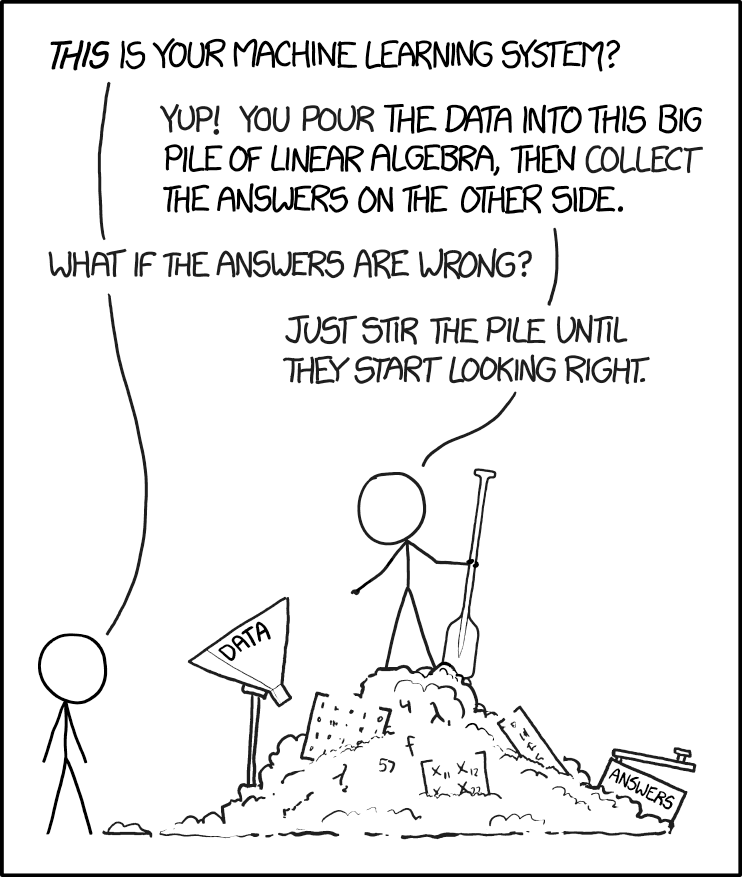
\includegraphics[width=0.5\linewidth]{xkcd/MachineLearning.png}
    \caption{\textbf{\href{https://xkcd.com/1838/}{Machine Learning}}}
\end{figure}
% add links to otehr things/useful external resoruces/using textbooks? 

\mychapter{4}{Problem Solving}
\epigraph{If you can't solve a problem, then there is an easier problem you can solve: find it.}
{\textit{George Pólya}}
% Include an example of how to understnad someting?
% Also cover things like comparing yourself to others and why that's not always useful? 

% Address the importance of strugling with problems - build onto the workshop section from before 

\section{Building the Toolkit}

% Talk about buildling that problem solving tooklit - then link to making notes? 

In this chapter, I want to challenge the idea that a Maths degree is just about learning more advanced techniques. 

If there’s one thing worth holding on to while studying mathematics, it’s that every definition, theorem, and technique exists because someone, at some point, was trying to solve a problem.

When you first meet a new topic, it can feel like a wall of definitions followed by results you’re expected to accept and apply. But mathematics did not begin as a fixed collection of rules. It began with curiosity. The ideas you learn were built to understand patterns, resolve contradictions, and make sense of problems that genuinely puzzled people. What you usually see at university is the finished structure, not the messy exploration that led to it. You won’t always see the motivation straight away and that’s normal. But it’s still worth remembering that the mathematics you’re learning exists because someone cared enough about a problem to keep thinking about it.

And in a way, that is what you are stepping into when you study mathematics. What this degree really develops is how you respond when you don’t immediately know what to do. It’s training you to sit with uncertainty without panicking, to break a large problem into smaller parts and identify structures where none seems obvious in the first glance. 

% If there's anythign you remember... rememebr that you do.. every theorem or formula you come across is because it was trying to solve some problem.. it’s not out of nowhere.. and once you think about maths as tools for solving problems.. intuition just falls out relatively easily… mathematician in the past had a reason ot be engaged in the problems, it wasn’t out of nowhere… so everything that you learn has a reason and has motivated people in the past.. that doesn’t mean you will appreciate all of them the same way ppl in the past did, but it does give you some reason and motivation to pursue studying this beautiful subject. 


When faced with something unfamiliar, mathematics teaches you to ask: 
\begin{itemize}
    \item What do I actually know? 
    \item What is the definition here? 
    \item What would have to be true for this to work? 
    \item Can I test a simpler example with numbers before generalising it? 
\end{itemize}


\subsection{Notes That Actually Help}
% Short-mid rant on what works/has worked in the past 
% Talk a bit about my own experience with note-taking?
% Depends on person, so encourage them to try something, see how useful that's been 
% best indicator usually - if you can explain it to someone else 
% sit down with the mindset that you will learn something new - and find that thing - treat lectures like exploration, because mathematics is exploration. 

You might spend the first few weeks trying to find the `right' way to take notes for something like Mathematics. Some people swear by handwriting because it slows them down, others type in \LaTeX \ or something else because it might be neater and easier to organise, some annotate the lecture slides or notes directly. There is no `one-size-fits-all' here. What works brilliantly for one person might be useless for another. 

The only reliable test is whether the system helps you think critically or not. If you find yourself with beautiful notes on the most recent Calculus lecture you attended but have no idea on how to approach the problem sheet, something needs to change. If you find not making any notes in lectures and reviewing information later in the evening helps ideas settle, try that. Or if you realise handwriting slows you down, see if you can find a way to condense information instead of copying a lot of things down. 

The goal here is not to produce the most elegant looking notes amongst your peers, but to build understanding that you can use for yourself. You are not being graded on your notes, but on your thinking, so ensure that the learning resources you use/build contribute to your thinking. 

\subsection{Explaining Things Out Loud}
% cite/reference the 'feynman' technique in the margin or something?

One habit that has helped me more than any particular note-taking method was explaining things out loud. 

A good test to see if you've understood something is usually later in the day or in the week, close your notes and try to explain the main idea either to a friend or out loud. 

You very quickly discover what you don't understand when you try to speak it. On paper, everything can look fine. But the moment you try to explain why some assumption is necessary, or why an implication follows, you feel the gap immediately. If you can explain a concept to someone else, even to an imaginary audience without constantly checking your notes, you are much closer to understanding a concept than if you simply reproduce what was written in the lecture. 
 

\section{What to Do When You're Stuck}

Problem solving sounds very inspiring until you're staring at Question 4 from Coursework 2 at 10:37pm or 38 minutes into the exam and your brain has gone offline. There will be moments in lectures or problem sheets or exams where you may genuinely not know how to begin. 

The instinct when stuck is often to rush, to scan the question faster or hope something jumps out. Instead, try and slow down. Read the question again. What is actually being asked? Rewrite the question in simpler terms and alongside it, any definitions or theorem you can recall about what is being asked. This does two things. First, it forces your brain back into structure and something you do know rather than panic. And secondly, everything that you need is given to you in the words of the question, and once you have unpicked the most important parts, you have part of a path forward. 

\section{On Gaining Insight}
% Need example of when I was really stuck on stuff 
\begin{quote}
One of the hardest things to unlearn at university is the urge to look at a solution the moment you feel stuck. Once you've seen someone else's solution, you can never recreate the benefit of discovering it yourself. Even if you don't solve the problem completely, struggling with it, forming wrong ideas, testing different approaches and hitting multiple dead ends does far more for your mathematical growth than neatly following a polished answer ever will.
\end{quote}

To illustrate this with an example, I remember getting stuck on a problem in my Linear Algebra II module that, in hindsight, was conceptually quite simple: showing that a certain set of functions formed a vector space. The technical details are not that important here.

On the one hand, I could've easily looked up the proof or asked AI to generate it in a few seconds, and it would probably have given me something correct and tidy. It might even have felt satisfying in the moment, but I suspect I would have mostly walked away with the illusion of understanding. 

Instead, I was in the workshop where I had my lecturer from the module present to talk me through the problem and refine the gaps in my thinking. Rather than being simply told what I had to write for the proof to fall out, we started from what I did know about the definition of additive identity and what it was supposed to satisfy, namely the condition $f +0 =f$, then treated this like an equation and worked out what this mysterious `zero function' would look like. 

Arriving at that idea, and more importantly, learning how to justify it properly, was the real insight. But that insight didn't come from seeing the finished proof, but from wrestling with the gap between knowing the definition and knowing how to write it in the abstract way the questions asked me to. Now, if I had skipped that part and just read up the solution, I would have `known' the answer, but would have lost the experience of learning how to reconstruct that kind of proof myself. 

And that's the difference. When you outsource your thinking, you might take pride in being incredibly efficient. But the price of efficiency is ownership, and the price of speed is insight, and with a subject as elegant and satisfying like Mathematics, that trade is just not worth it. 

\section{Why This Matters}

This reason these problem solving skills matter is not because you will be constantly proving theorems outside university. It matters because the habits transfer. Learning how to decompose complex problems into manageable parts, staying calm under uncertainty, testing assumptions, communicating reasoning clearly. These are all thinking skills that reshape how you approach problems in the real world. 


\begin{figure}[H]
    \centering
    \begin{minipage}{0.48\linewidth}
        \centering
        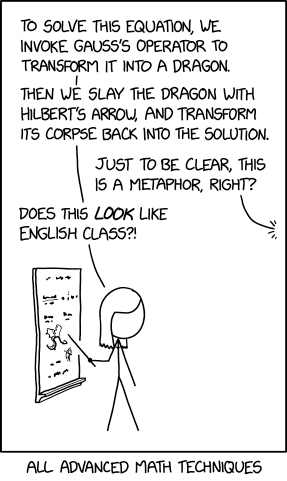
\includegraphics[width=\linewidth]{xkcd/advancedTechniques.png}
        \caption{\textbf{\href{https://xkcd.com/2595/}{Advanced Techniques}}}
    \end{minipage}
    \hfill
    \begin{minipage}{0.48\linewidth}
        \centering
        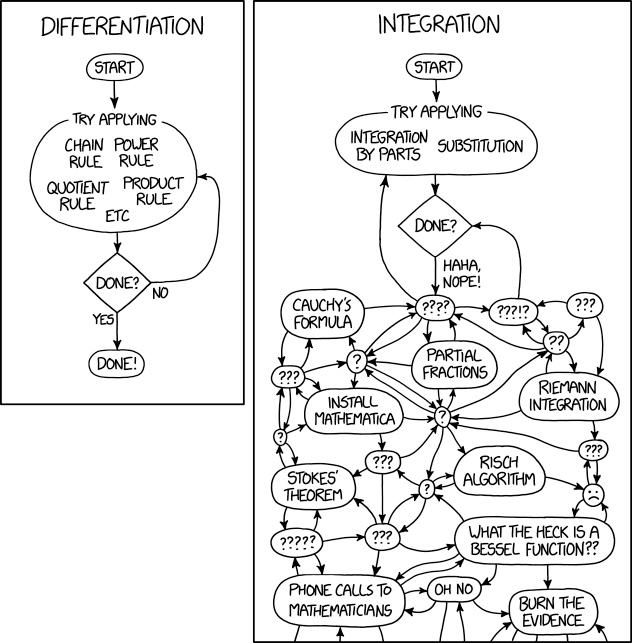
\includegraphics[width=\linewidth]{xkcd/integration.png}
        \caption{\textbf{\href{https://xkcd.com/2117/}{Differentiation and Integration}}}
    \end{minipage}
\end{figure}

\mychapter{5}{Exams}
\epigraph{The epigraph for this chapter is left as an exercise to the reader}{}


\section{Structure of Assessments}

% How exams work - when they are - what are the weights of assessments and grades like? Subject to change per year so look at module informatio on blackboard 

% how to manage revision - asking for help, etc. 

% Speical cons policy for exams - add links 

% Mid-terms and finals 

Assessment in the first year is usually a mixture of coursework and written or online exams. The exact weighting varies between modules, so it’s always worth checking the information provided on Blackboard or the module page at the start of the semester. Lecturers will usually explain the assessment structure in the first few weeks of the module as well.

All first year modules also have a written in-person exam at the end of the semester. These typically take place during the university’s official exam periods which is in January for Semester 1 modules and in the summer for Semester 2 modules.

\section{Revision}
% how to revise well for something like maths? signpost to student hub learning skills and confidence and other helpful stuff available at uni. 

\subsection{Using Past Papers}
% how to use past papers effectivley? - don't just have the solutions as you do the papers, cuz there are dangers to that 
% tips for multiple choice - eliminate options 
% once you look at the solution, don't just gloss over it 
% also, don't rely on it as the only form of revision 

Past papers are one of the most useful revision tools you have, but also one of the easiest to misuse. 

It's very tempting to just load up a paper, try a question for a few minutes, get stuck, look at the solution, understand it and move on. The most important thing is to give yourself time to think before reaching for help. So if and when you don't know how to start a question, sit with it for a bit. Even if you don't solve it completely, that thinking time matters and it's what builds the ability to approach unfamiliar problems. 

If you look at a solution, try to reconstruct the proof yourself without looking. If you can't, that's a sign you didn't fully understand it yet, and that's fine. 

Try to not let past papers become the syllabus. It can be easy to fall into the habit of revision from the papers instead of using them as a tool to test your understanding. Exams don't always test whether you've seen a question before, but whether you understand the material well enough to deal with something slightly unfamiliar. So if your revision is entirely based on past papers, a small variation in a problem can make it feel like you've never seen it before.

\subsection{Dealing with Stress}
% Shakespeare in love - philip henslowe
% What to do if you're bored in an exam/deal with not wantiang to be there? 
% What to do if you're stressed the hell out in the exam

There is a particular kind of stress that arrives a few days before exams begin, and it’s not really about content. It’s about doubt.

You start asking questions that don’t have neat answers. Have I revised enough? What if I’ve focused on the wrong topics? What if the paper goes badly? What if I’ve misunderstood something fundamental? What if…? what if…? what if…? 

The mind becomes very creative under pressure. At some point it stops being about mathematics and starts being about catastrophe. Exam stress, dread, and self doubt are incredibly common, especially among people who care deeply about their subject. But even knowing that, it’s easy to feel alone when you’re in the middle of it.

I remember feeling this intensely before my first January exams in Semester 1. I was convinced I hadn’t done enough, that I was about to fail half my modules, and those thoughts seemed to be louder than any rational argument I could make.

I fondly remember speaking to my tutor about how stressed I was, and one of the first things he said to me was: 

\begin{quote}
    \textit{''It’s gonna to be alright. I’m not saying you’re gonna feel alright about it. I’m just saying it’s gonna to be alright."}
\end{quote}

I asked him how he knew, to which would response was, \textit{``How? I don’t know. It’s a mystery."}

Then he showed me a \textbf{\href{https://youtu.be/-hxTrm34oRI?si=08GXYMDkDqyzMvLp}{clip from Shakespeare in Love}}, where Philip Henslowe says exactly that line when everything seems to be falling apart.

Watching an 18 second YouTube video wasn’t exactly the kind of reassurance I expected going into that conversation, but there was something oddly comforting about that phrase. Something about it stayed with me, and it wasn’t because it removed the stress (it didn’t) but rather that it removed the demand to know, to predict, to control. It wasn’t saying I wouldn’t worry, but that uncertainty doesn’t mean catastrophe.

Later that evening, I printed out the script from Shakespeare in Love and put it on my wall. Since then, every time my mind started racing or I felt like I was catastrophising scenarios, I would look at it and smile, slightly against my will.

I don’t think the lesson here is that exams should feel easy, or that stress can be eliminated entirely. The lesson, at least for me, was simpler than that.

You revise as well as you can, sit the paper, and attempt the questions in front of you with whatever you can bring to mind that day.

Going in with that mindset feels very different from walking into the exam convinced you’re either going to ace everything, or on the flip side convinced you’re going to fail everything. Both extremes are unhelpful: one sets you up for pressure, the other for panic. 

Whereas if you accept that you don’t know exactly how it will go, and that you might surprise yourself in either direction, you can focus on thinking clearly instead of predicting the outcome.

And once the paper leaves your hands, some part of it really is a mystery.



\subsection{Comparison}
% This is not a rat race, cooperation over comparison or whatever else... talk abotu how comparison can cause anxiety, especially with Maths 

Comparison is one of the fastest ways to drain your confidence during revision. 

You will overhear conversations about how much or how many hours someone else has done, see people in the library morning to night, or someone say how they've completed every past paper twice. 

None of that gives you actual useful information. You don't know how well they understood the material, or what their starting point was, or even whether what they are telling you is the entire truth or only a fraction of it. 

The only revision that matters is yours. There will always be someone who appears more prepared, more calmer, or understands things instantly. Just because someone else appears better or smarter than you, doesn't make you any more or less good. Someone else understanding a concept quickly does not make you any less capable. 

The person who seems completely calm might also be unsure, and the student who answers questions confidently in lectures might have struggled with a different topic entirely. Nobody every has it `all worked out'. Comparison is always based on partial information, you rarely get to see the full picture. And during revision when anxiety and adrenaline are already elevated, comparison amplifies doubt without adding any insight. 

Mathematics is not a race in a straight line. Intellectual growth is personal, and often invisible. So let other people exist, let them be brilliant and revise in their way. You task is not to outperform everyone, but to engage the best you can with the material in front of you. 

\section{Results}
% in case things don't go according to plan - link to special cons. 
% Summer resits and criteria around that - add links to relevant things. 
% How first year grades don't count towards final degree- you just need to pass so don't stress too much blah blah blah - it's not an exuces for doing badly and not showing up to lectures tho 

% Section on addressing imposter syndrome thoughts like, “oh I don’t deserve these results because I didn’t work hard enough” and on the flip side, “I worked so hard only to get these low grades I'm terrible” 

During exams you’re busy thinking, writing, calculating, trying to make sense of questions under time pressure. But once the results come out, the thinking changes. You’re no longer solving problems but instead interpreting a number and trying to decide what it means about you.

The reaction to good results isn’t always excitement, sometimes it’s thoughts like  `Did I actually deserve that?' Or `I didn’t work hard enough to deserve that grade'. It’s that strange feeling of somehow getting away with something.

If you’ve ever had that thought, you’re not alone. Mathematics has a way of making people doubt themselves even when things go well. The subject constantly shows you how much more there is to learn, so it’s easy to feel like you’re always a step behind. But you’re allowed to accept the result you earned, you’re allowed to have done better than you expected.

The opposite reaction can happen too. Sometimes you work incredibly hard and the result feels disappointing and that can be much harder to process. When you’ve put hours into something, it’s easy to let one number turn into a judgement about your ability.

That voice can be very convincing in the moment. Remember that results are merely a snapshot of how things went in a particular exam, on a particular day, under particular conditions. It’s easy to believe that the world is like a neat function, that the effort your input always results in the outcome you want, but the world is uncertain and full of variables beyond our control. That doesn’t mean your effort was wasted, it just means your effort isn’t the only deciding factor, and it definitely doesn’t mean your worth is defined by one exam or one outcome. 

In first year especially, it’s worth keeping a bit of perspective. The marks from first year don’t count towards your final degree as long as you pass the modules. Now, that doesn’t mean the year doesn’t matter. It absolutely does, in fact, it’s where a lot of the real learning happens and it does count for any placements or internships you might want to apply. But it does mean the stakes aren’t quite as catastrophic as your brain might try to convince you.

If things genuinely don’t go according to plan, there are formal processes in place like summer resits, \textbf{\href{https://www.southampton.ac.uk/studentservices/academic-life/special-considerations.page}{special considerations}}, etc. It’s always worth checking in with your tutor following results if you find yourself in that situation. 


\begin{figure}[H]
    \centering
    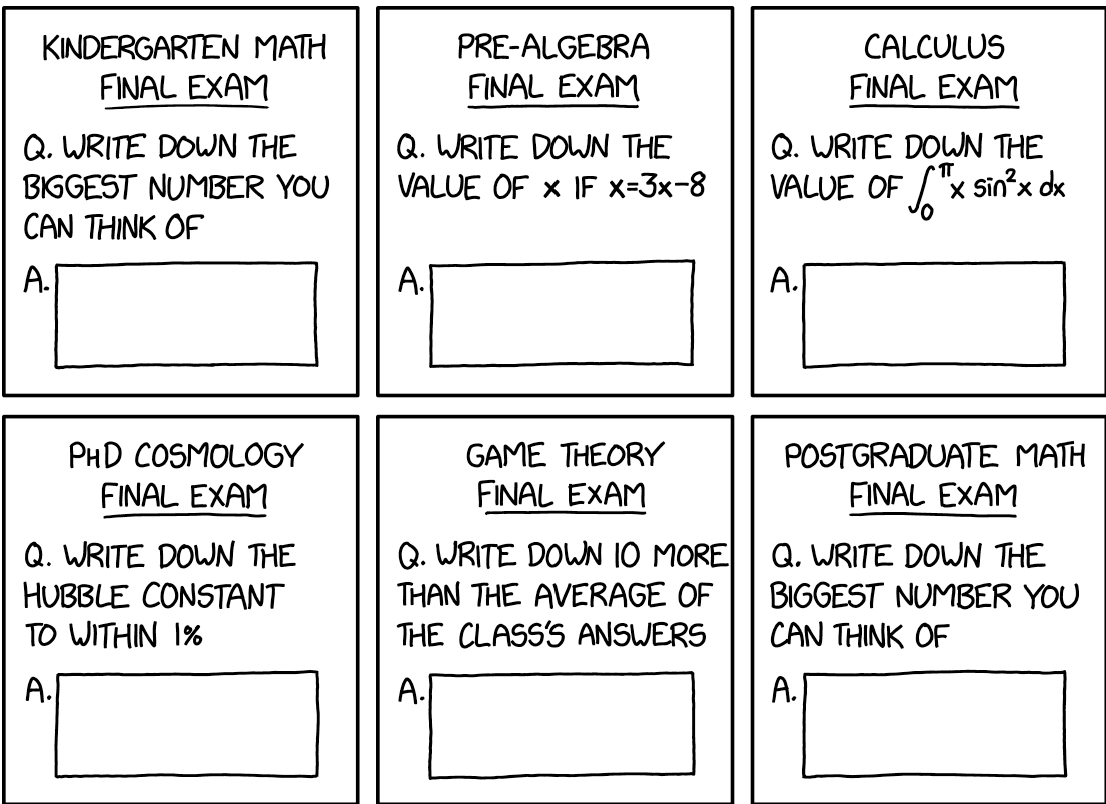
\includegraphics[width=0.5\linewidth]{xkcd/examNumbers.png}
    \caption{\textbf{\href{https://xkcd.com/2966/}{Exam Numbers}}}
\end{figure}


\begin{figure}[H]
    \centering
    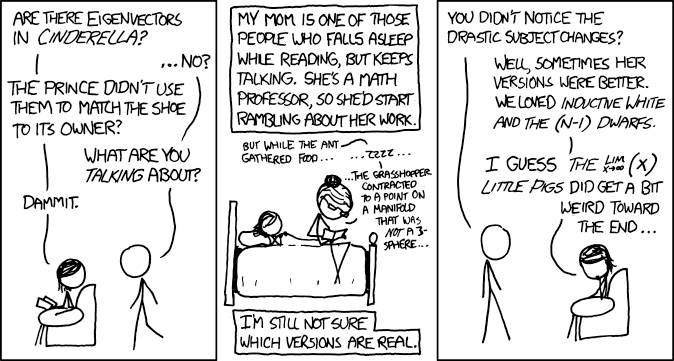
\includegraphics[width=0.6\linewidth]{xkcd/fairyTales.png}
    \caption{\textbf{\href{https://xkcd.com/872/}{Fairy Tales}}}
\end{figure}

\mychapter{6}{Time Management}
\epigraph{The bad news is time flies. The good news is you're the pilot}
{\textit{Michael Altshuler}}

% There is more to life than just maths basically

% Take up other things - exericse - join socieits - univeristy has so many things to offer - learn how to cook - spend time with friends 

% Continue hobbies 

% How to deal with things overhwelmign and burn out 


\section{Structuring Time}

There is a funny shift that happens in the first few weeks of university. No-one tells you what to do between lectures. 

You might have three lectures in the morning and then nothing scheduled until the following afternoon. That looks like a lot of free time but in reality, it's hours of unstructured time. And unstructured time has a habit of disappearing. 

Time management in a Maths degree isn’t about cramming more hours in, but about avoiding last-minute panic. Maths needs uninterrupted thought. One hour of undistracted thinking is worth more than three hours of broken attention. If you have a two hour gap between lectures, don't assume it's automatically productive time. Decide in advance what you're going to go. Sometimes you might be tired and use that to relax and read a novel or a hit the gym, or maybe you didn't quite understand the last 10 mins of the previous lecture and want to review the notes. It doesn't matter what you do, as long as it's intentional. 

\section{Overworking vs Avoidance}

It’s easy to confuse burnout with avoidance. If you are avoiding starting because the work feels uncomfortable, that’s one thing. Usually once you begin, the momentum builds. However, if you're staring at the page feeling exhausted and unable to process even simple steps, that’s something else. 

Being honest about which one you are experiencing is important. There is no pride in pushing through exhaustion just to prove you can, and equally, there is no growth in endlessly procrastinating out of fear.

If you find yourself consistently overwhelmed, talk to someone. That could be your personal tutor, the \textbf{\href{https://www.southampton.ac.uk/studentservices/support-wellbeing.page}{Student Hub wellbeing team}}, the \textbf{\href{https://www.susu.org/support/university-support.html}{SUSU advice centre}}, or even your friends. University has systems in place because they know how common it is for students to struggle with these things.  

\section{Life Outside the Degree} 

It can be quite easy for your degree to consume everything. And sometimes that feels good, but remember that university is not just a degree factory. 

There are lots of \textbf{\href{https://www.susu.org/activities/}{clubs and societies}}, sports, random Wednesday evenings that end up in unexpectedly good memories. Making time and space for those things is part of the experience, not a distraction. 

I have always found that I think more clearly after stepping away from a problem having spent a considerable amount of time on it. Some of the best insights into problems and questions arrived while I was engaged in something else entirely like cooking or rowing. 

There will be weeks where the workload increases and the social things need to take a slight step back, and there will also be weeks where you might say yes to more events outside of academics. Whatever it might be, balance is not something you're expected to achieve once and then maintain perfectly, it requires constant adjustment. 

If you’re always exhausted, something needs to change. If you’re always disengaged, something also needs to change. Doing a maths degree can feel intense at times as it demands genuine critical thinking. But it still is a degree, not your entire identity. So work hard, and also remember to close the notebook sometimes and have fun. 




\begin{figure}[H]
    \centering
    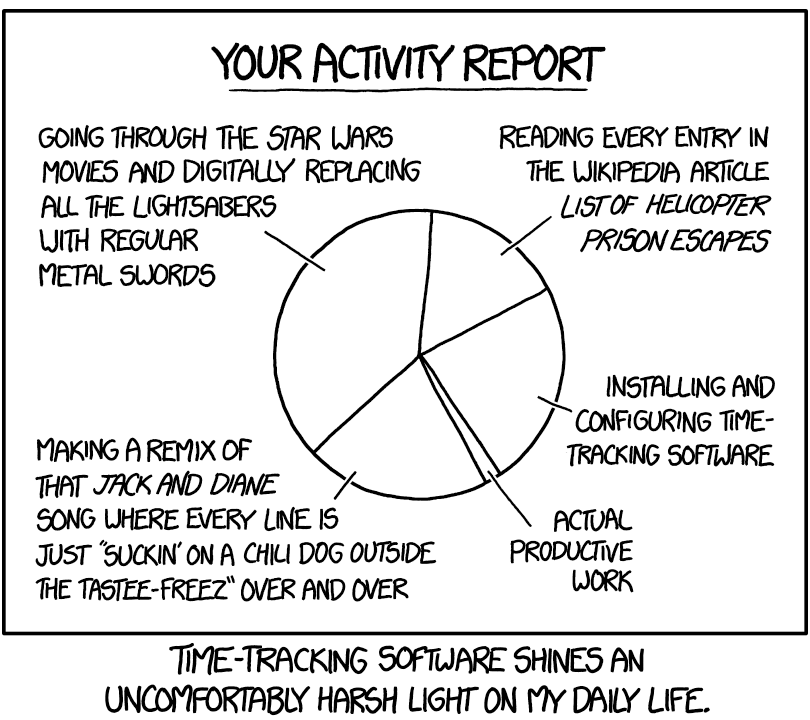
\includegraphics[width=0.5\linewidth]{xkcd/timeTracking.png}
    \caption{\textbf{\href{https://xkcd.com/1690/}{Time-Tracking Software}}}
\end{figure}

\begin{figure}[H]
    \centering
    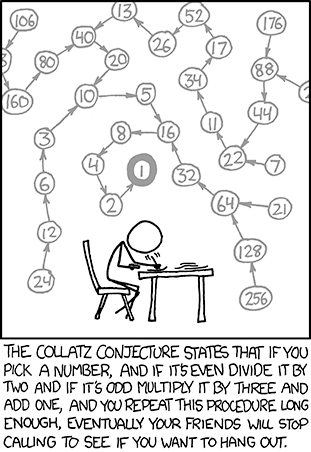
\includegraphics[width=0.4\linewidth]{xkcd/collatzConjecture.png}
    \caption{\textbf{\href{https://xkcd.com/710/}{Collatz Conjecture}}}
\end{figure}



\mychapter{7}{Common Terms, Abbreviations, and Useful Links}
\epigraph{An undefined term is the beginning of every definition}
{\textit{Bertrand Russell}}

Throughout this guide, a number of links, terms, and abbreviations come up repeatedly, which are now collated here for reference. 

\textbf{\href{https://www.southampton.ac.uk/studentservices/index.page}{The Student Hub}} \\
24/7, first point of contact support service for students providing advice and guidance on things like wellbeing, finance, accommodation, etc. 

\textbf{\href{https://sotonac.sharepoint.com/}{SUSSED}} \\
The University's main intranet portal used by students and staff for news, updates, events, and quick links to key services. 

\textbf{\href{https://www.southampton.ac.uk/about/faculties-schools-departments/school-of-mathematical-sciences}{School of Mathematical Sciences}} 

\textbf{\href{https://www.southampton.ac.uk/studentadmin/academic-support-guidance/personal-tutor.page}{PAT}} - Personal Academic Tutor \\  
A member of staff who will help you settle in your studies, support your academic progress and act as a key contact for queries, or direct you to other support services if you need it. 

\textbf{Office Hours}\\
Designated times when lecturers are available for students to drop by to discuss academic content, feedback, or module-related questions outside of scheduled lectures. 

\textbf{\href{https://library.soton.ac.uk/feedback/types}{Formative and Summative Assessments}}\\
Formative mark doesn’t to count towards your final mark for the module; summative counts towards the final mark.

\textbf{Accreditations} \\
Actuarial science programmes at the University of Southampton are accredited by the \textbf{\href{https://actuaries.org.uk/}{Institute and Faculty of Actuaries (IFoA)}}, allowing students to gain exemptions from core principles examinations (CS1, CS2, CM1, CM2, CB1, CB2). Key accredited programs include BSc Mathematics with Actuarial Science and BSc Economics and Actuarial Science. For further details, contact Actuarial Sciences course lead. 

\textbf{\href{https://www.southampton.ac.uk/about/governance/regulations-policies/taught-students/general/credit-accumulation-transfer}{CATS/ECATS}}\\
Systems used to measure and transfer academic credit for modules and degrees.

\textbf{\href{https://www.southampton.ac.uk/quality/governance/sslctaught.page}{SSLC}} - Student Staff Liaison Committee \\
Meeting where student representatives and academic staff discuss and resolve issues, enhancing the overall education and student experience

\textbf{\href{https://www.susu.org/representation/academic-representation.html}{Course and Academic Reps}} \\
Students volunteers who collect feedback on teaching, learning, and assessments to improve the student experience and liaise with staff in SSLCs. 

\textbf{\href{https://www.susu.org/}{SUSU}} - Southampton University Student Union \\
A student-led organisation independent from the university that is run by students, for students. 

\textbf{\href{https://www.susu.org/groups/sums}{SUMS}} - Southampton University Maths Society 

\textbf{\href{https://www.susu.org/groups/suas}{SUAS}} - Southampton University Actuarial Society 

\textbf{\href{https://www.southampton.ac.uk/library/index.page}{Library Services}}
 
\textbf{\href{https://library.soton.ac.uk/sash}{Library - Academic Skills Service}}

\textbf{\href{https://www.southampton.ac.uk/student-life/accommodation}{Student Accommodation}}

\textbf{\href{https://store.southampton.ac.uk/short-courses/halls/student-experience-engagement/kitchen-school}{Kitchen School}} \\
A hands-on, expert-led cookery program for students designed to teach basic culinary skills, healthy cooking, and food safety. 

\begin{figure}[H]
    \centering
    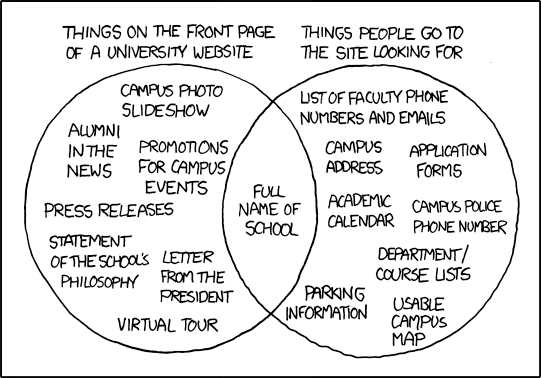
\includegraphics[width=0.6\linewidth]{xkcd/uniWebsite.png}
    \caption{\textbf{\href{https://xkcd.com/773/}{University Website}}}
\end{figure}

\begin{figure}[H]
    \centering
    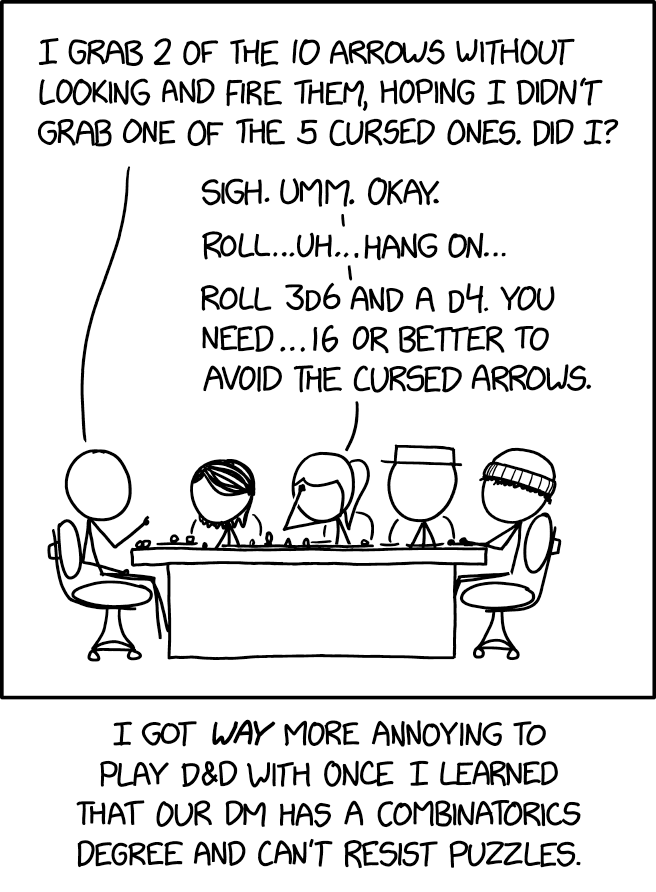
\includegraphics[width=0.5\linewidth]{xkcd/dnd.png}
    \caption{\textbf{\href{https://xkcd.com/3015/}{DnD Combinatorics}}}
\end{figure}

% make sure all relevant links exist/write a short des. for each? 


\listoffigures


\end{document}
